%!TEX root = ../paper.tex
\begin{figure}[!ht]
\centering
\noindent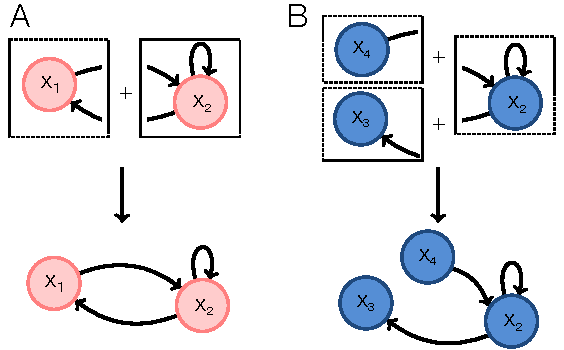
\includegraphics[width=0.4\columnwidth]{fig/examplesystemmodules.pdf}
\caption{{\bf Example of the combination of open system modules to construct closed systems.} (A) Example of combining two open modules to construct a closed system of two components (B) Analogous example for combining three open modules to construct a closed system with three components}
\label{fig:examplesystemmodules}
\end{figure}

\pagebreak

\begin{figure}[!ht]
\centering
\noindent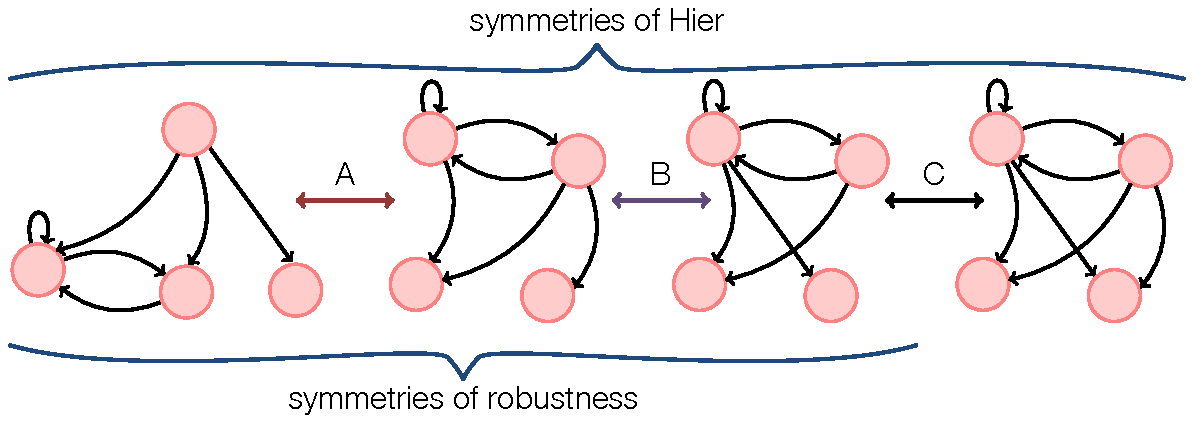
\includegraphics[width=0.7\columnwidth]{fig/hiertransformations.pdf}
\caption{{\bf Symmetries of the $\hier$ transformation between graphs and SCCs.} The transformation A represents an interchange of SCCs, B moving a link between nodes in a component and C adding a link. All three transformations represent symmetries of the $\hier$ transformation from graphs to SCCs while only A and B are symmetries of robustness.}
\label{fig:hiertransformations}
\end{figure}

\pagebreak

\begin{figure}[!ht]
\centering
\noindent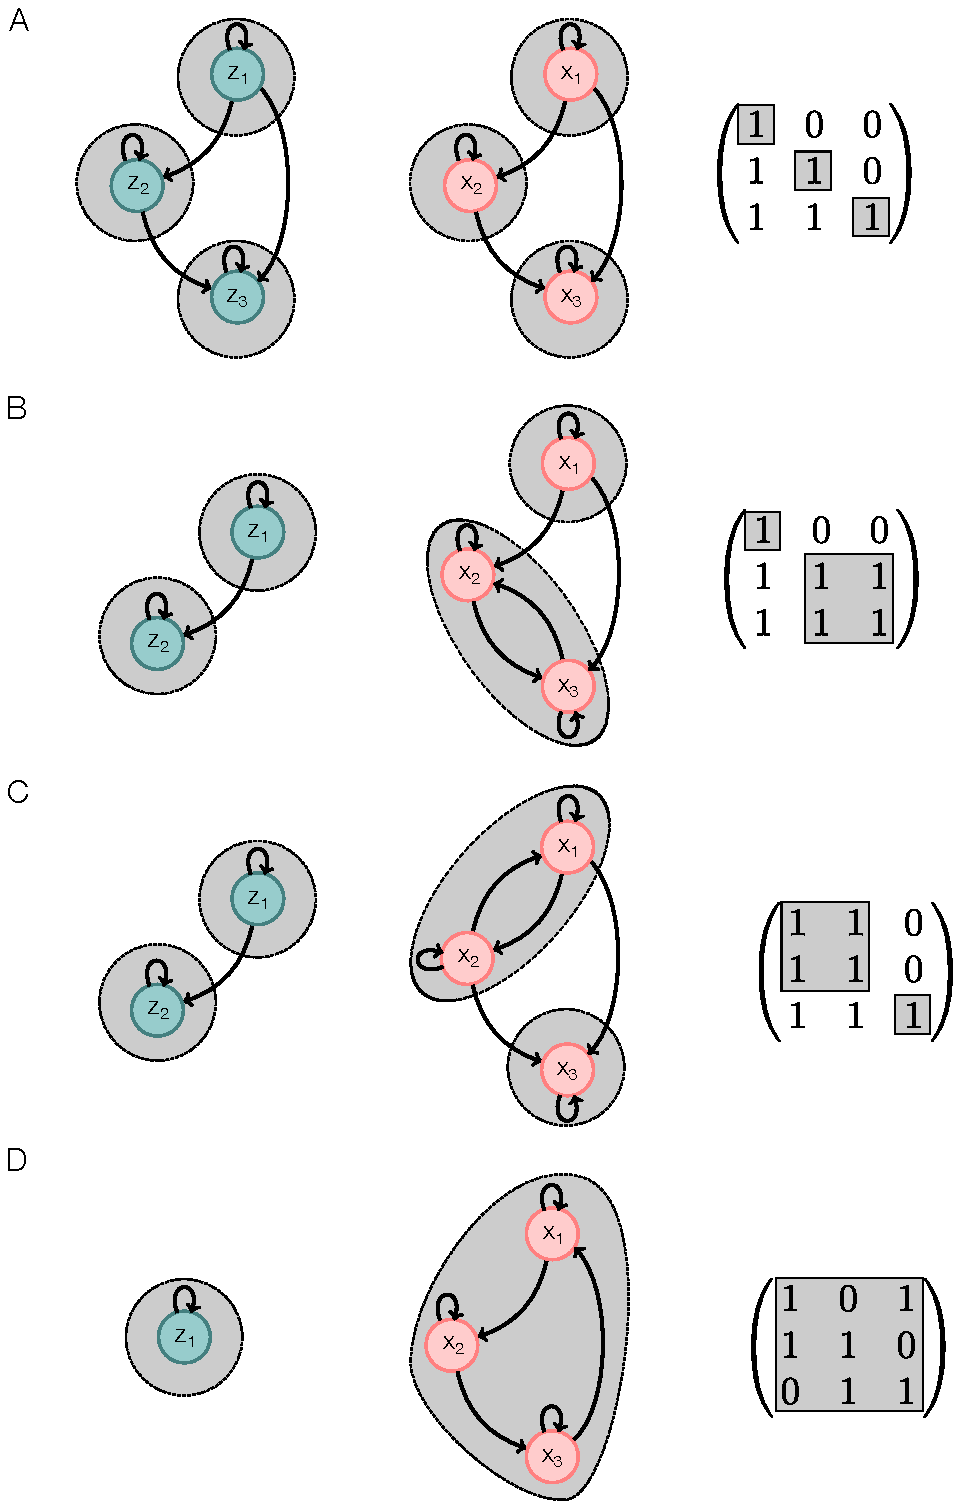
\includegraphics[width=0.4\columnwidth]{fig/scc2.pdf}
\caption{{\bf Example of strongly connected components.} (A) - (D) show strongly connected components highlighted in gray for each of the four graphs representing the interdependencies relevant to four different three component systems. Note that the most hierarchical system in (A) has the highest possible number of connected components, three, whereas the system containing a single cycle and therefore posessing no hierarchy contains only one connected component. Systems (B) and (C) represent examples of hierarchical modular systems that posess both modularity and hierarchy.}
\label{fig:scc}
\end{figure}

\pagebreak

\begin{figure}[!ht]
\centering
\noindent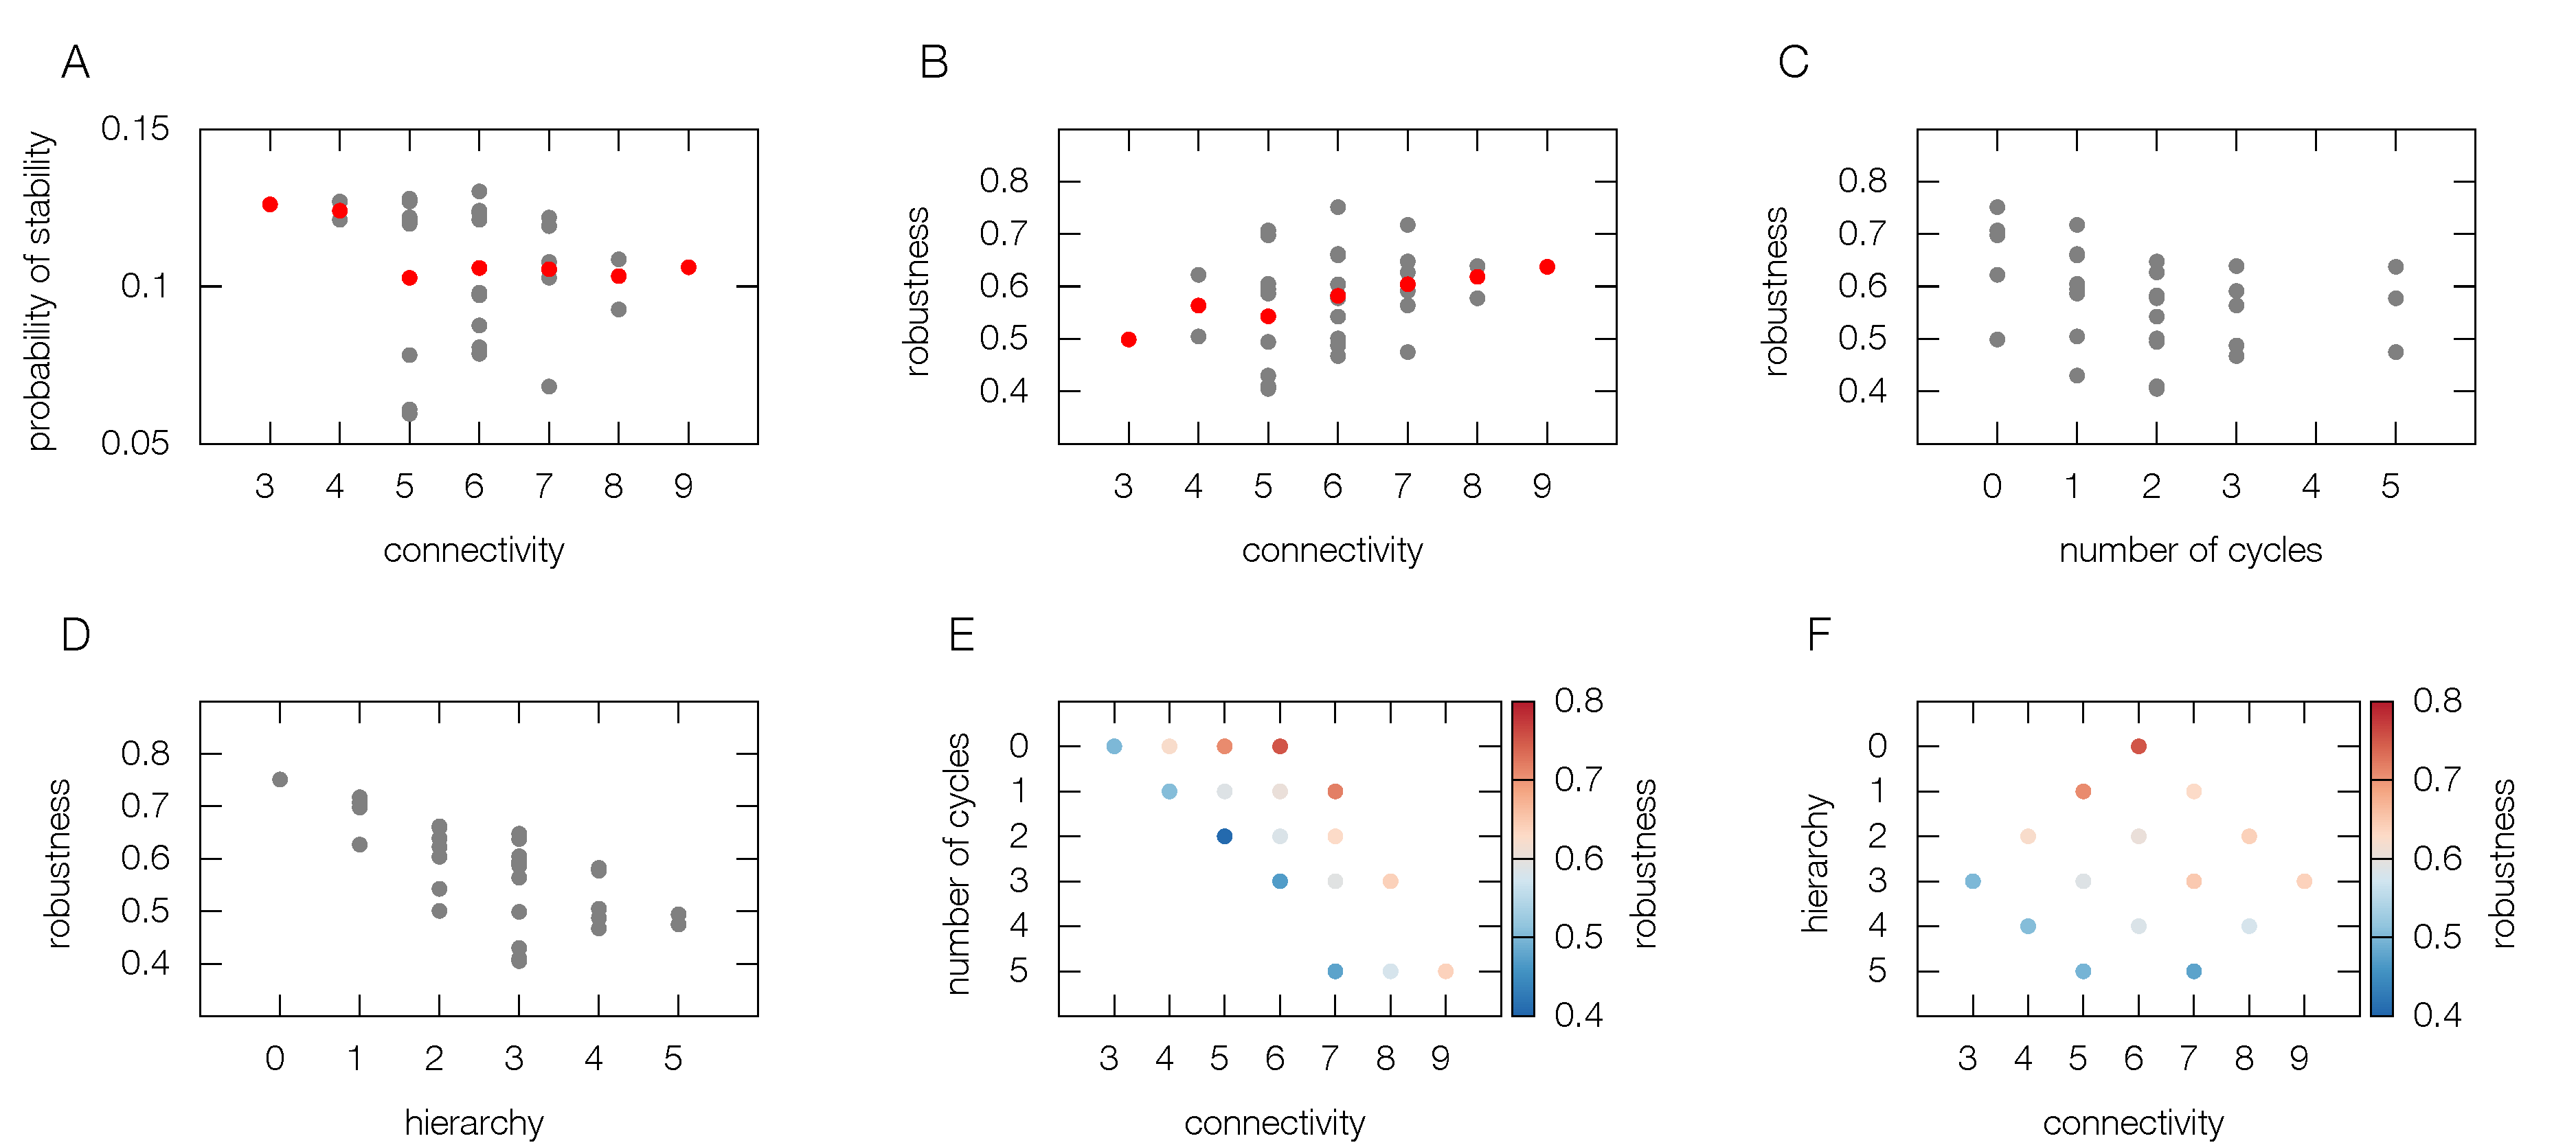
\includegraphics[width=1.0\columnwidth]{fig/combinedfigs.pdf}
\caption{{\bf Characterization of stability and robustness according to properties of system structure} (A) Stability versus connectivity, (B) robustness versus connectivity, (C) robustness versus number of cycles, (D) robustness versus hierarchy%, (E) robustness versus number of cycles and connectivity, and (F) robustness versus graph edit distance and connectivity
 for three component systems.
}
\label{fig:combined}
\end{figure}

% Figure translations
% apstab3x3 4 -> A
% stab3x3 6 -> B
% cycle3x3 7 -> C
% New -> D
% connectcycle3D3x3 5 -> E
% New -> F

% \begin{figure}[!ht]
% \centering
% \noindent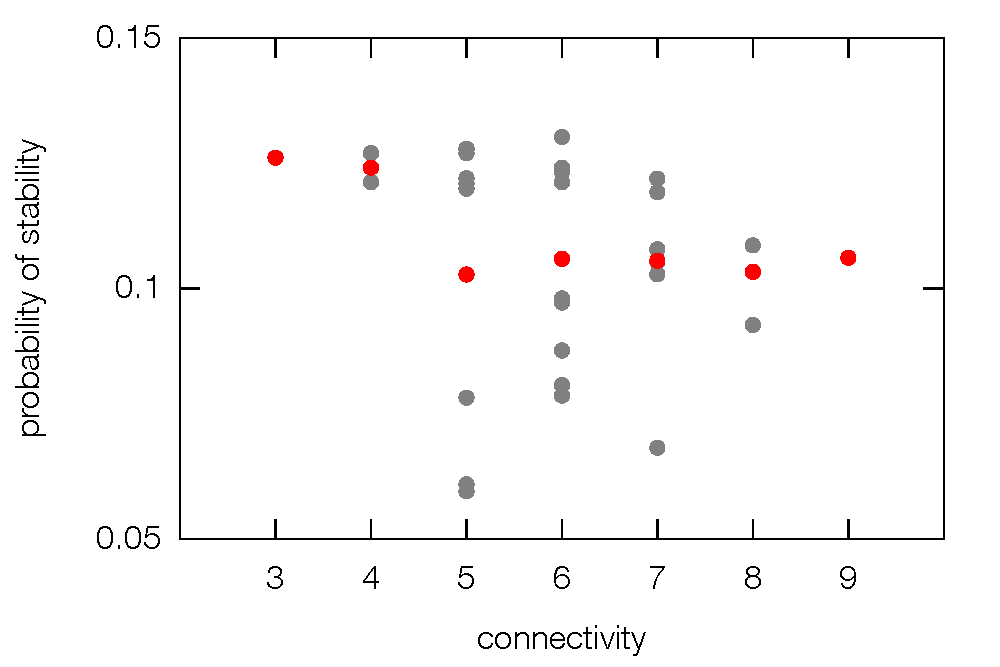
\includegraphics[width=0.8\columnwidth]{fig/apstab3x3.pdf}
% \caption{{\bf Plot of stability versus connectivity for three component systems.} }
% \label{fig:apstab3x3}
% \end{figure}

\pagebreak

\begin{figure}[!ht]
\centering
\noindent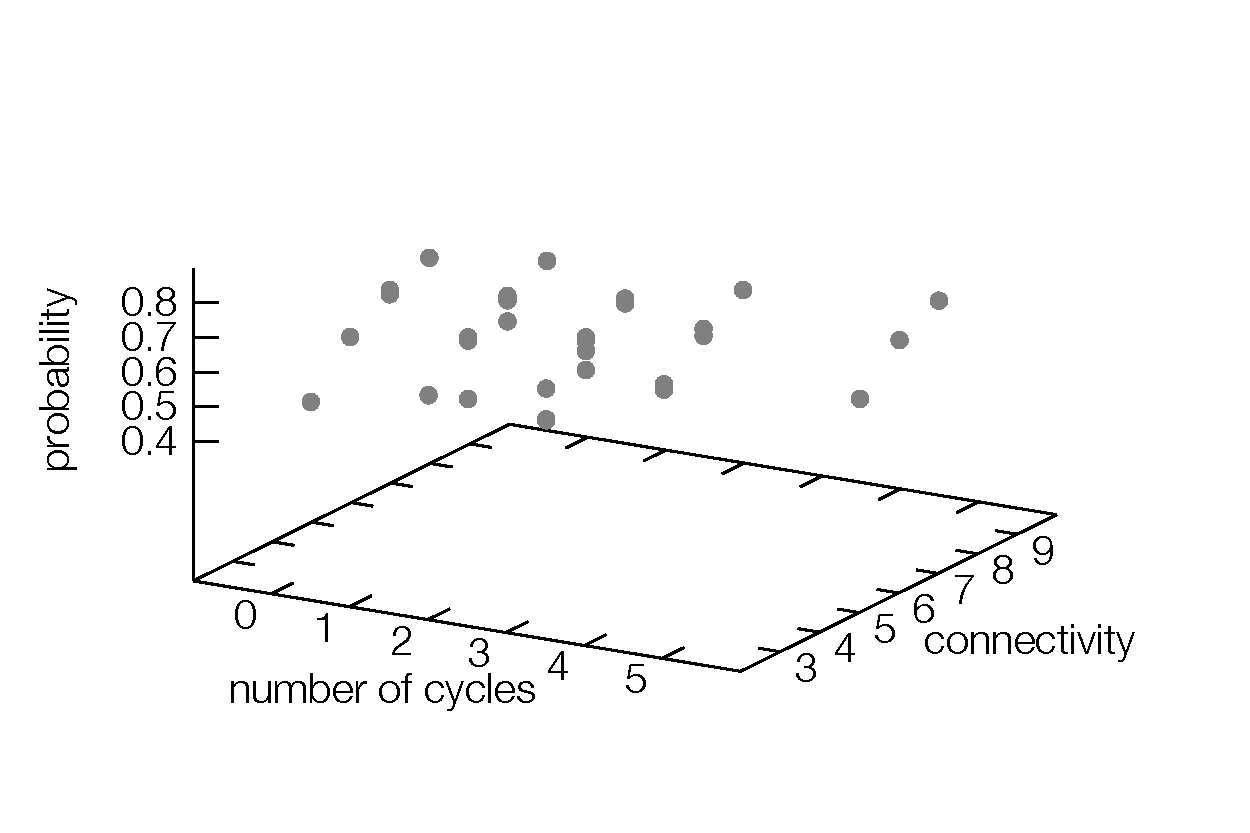
\includegraphics[width=0.7\columnwidth]{fig/connectcycle3D3x3.pdf}
\caption{{\bf Stability to perturbations versus number of cycles and connectivity for three component systems.} }
\label{fig:connectcycle3D3x3}
\end{figure}

\pagebreak

\begin{figure}[!ht]
\centering
\noindent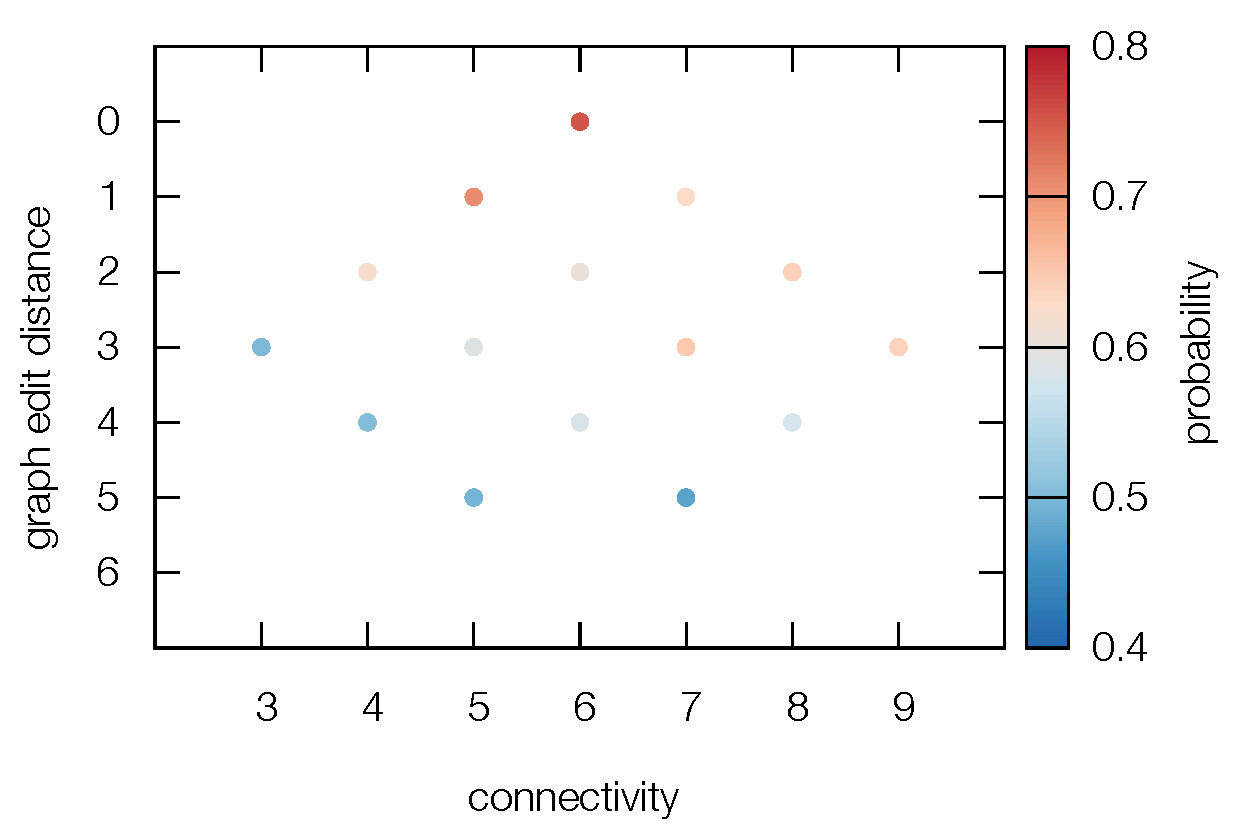
\includegraphics[width=0.7\columnwidth]{fig/connectdist3D3x3.pdf}
\caption{{\bf Robustness versus hierarchy and connectivity for three component systems.} }
\label{fig:connectdist3D3x3}
\end{figure}

\pagebreak

\begin{figure}[!ht]
\centering
\noindent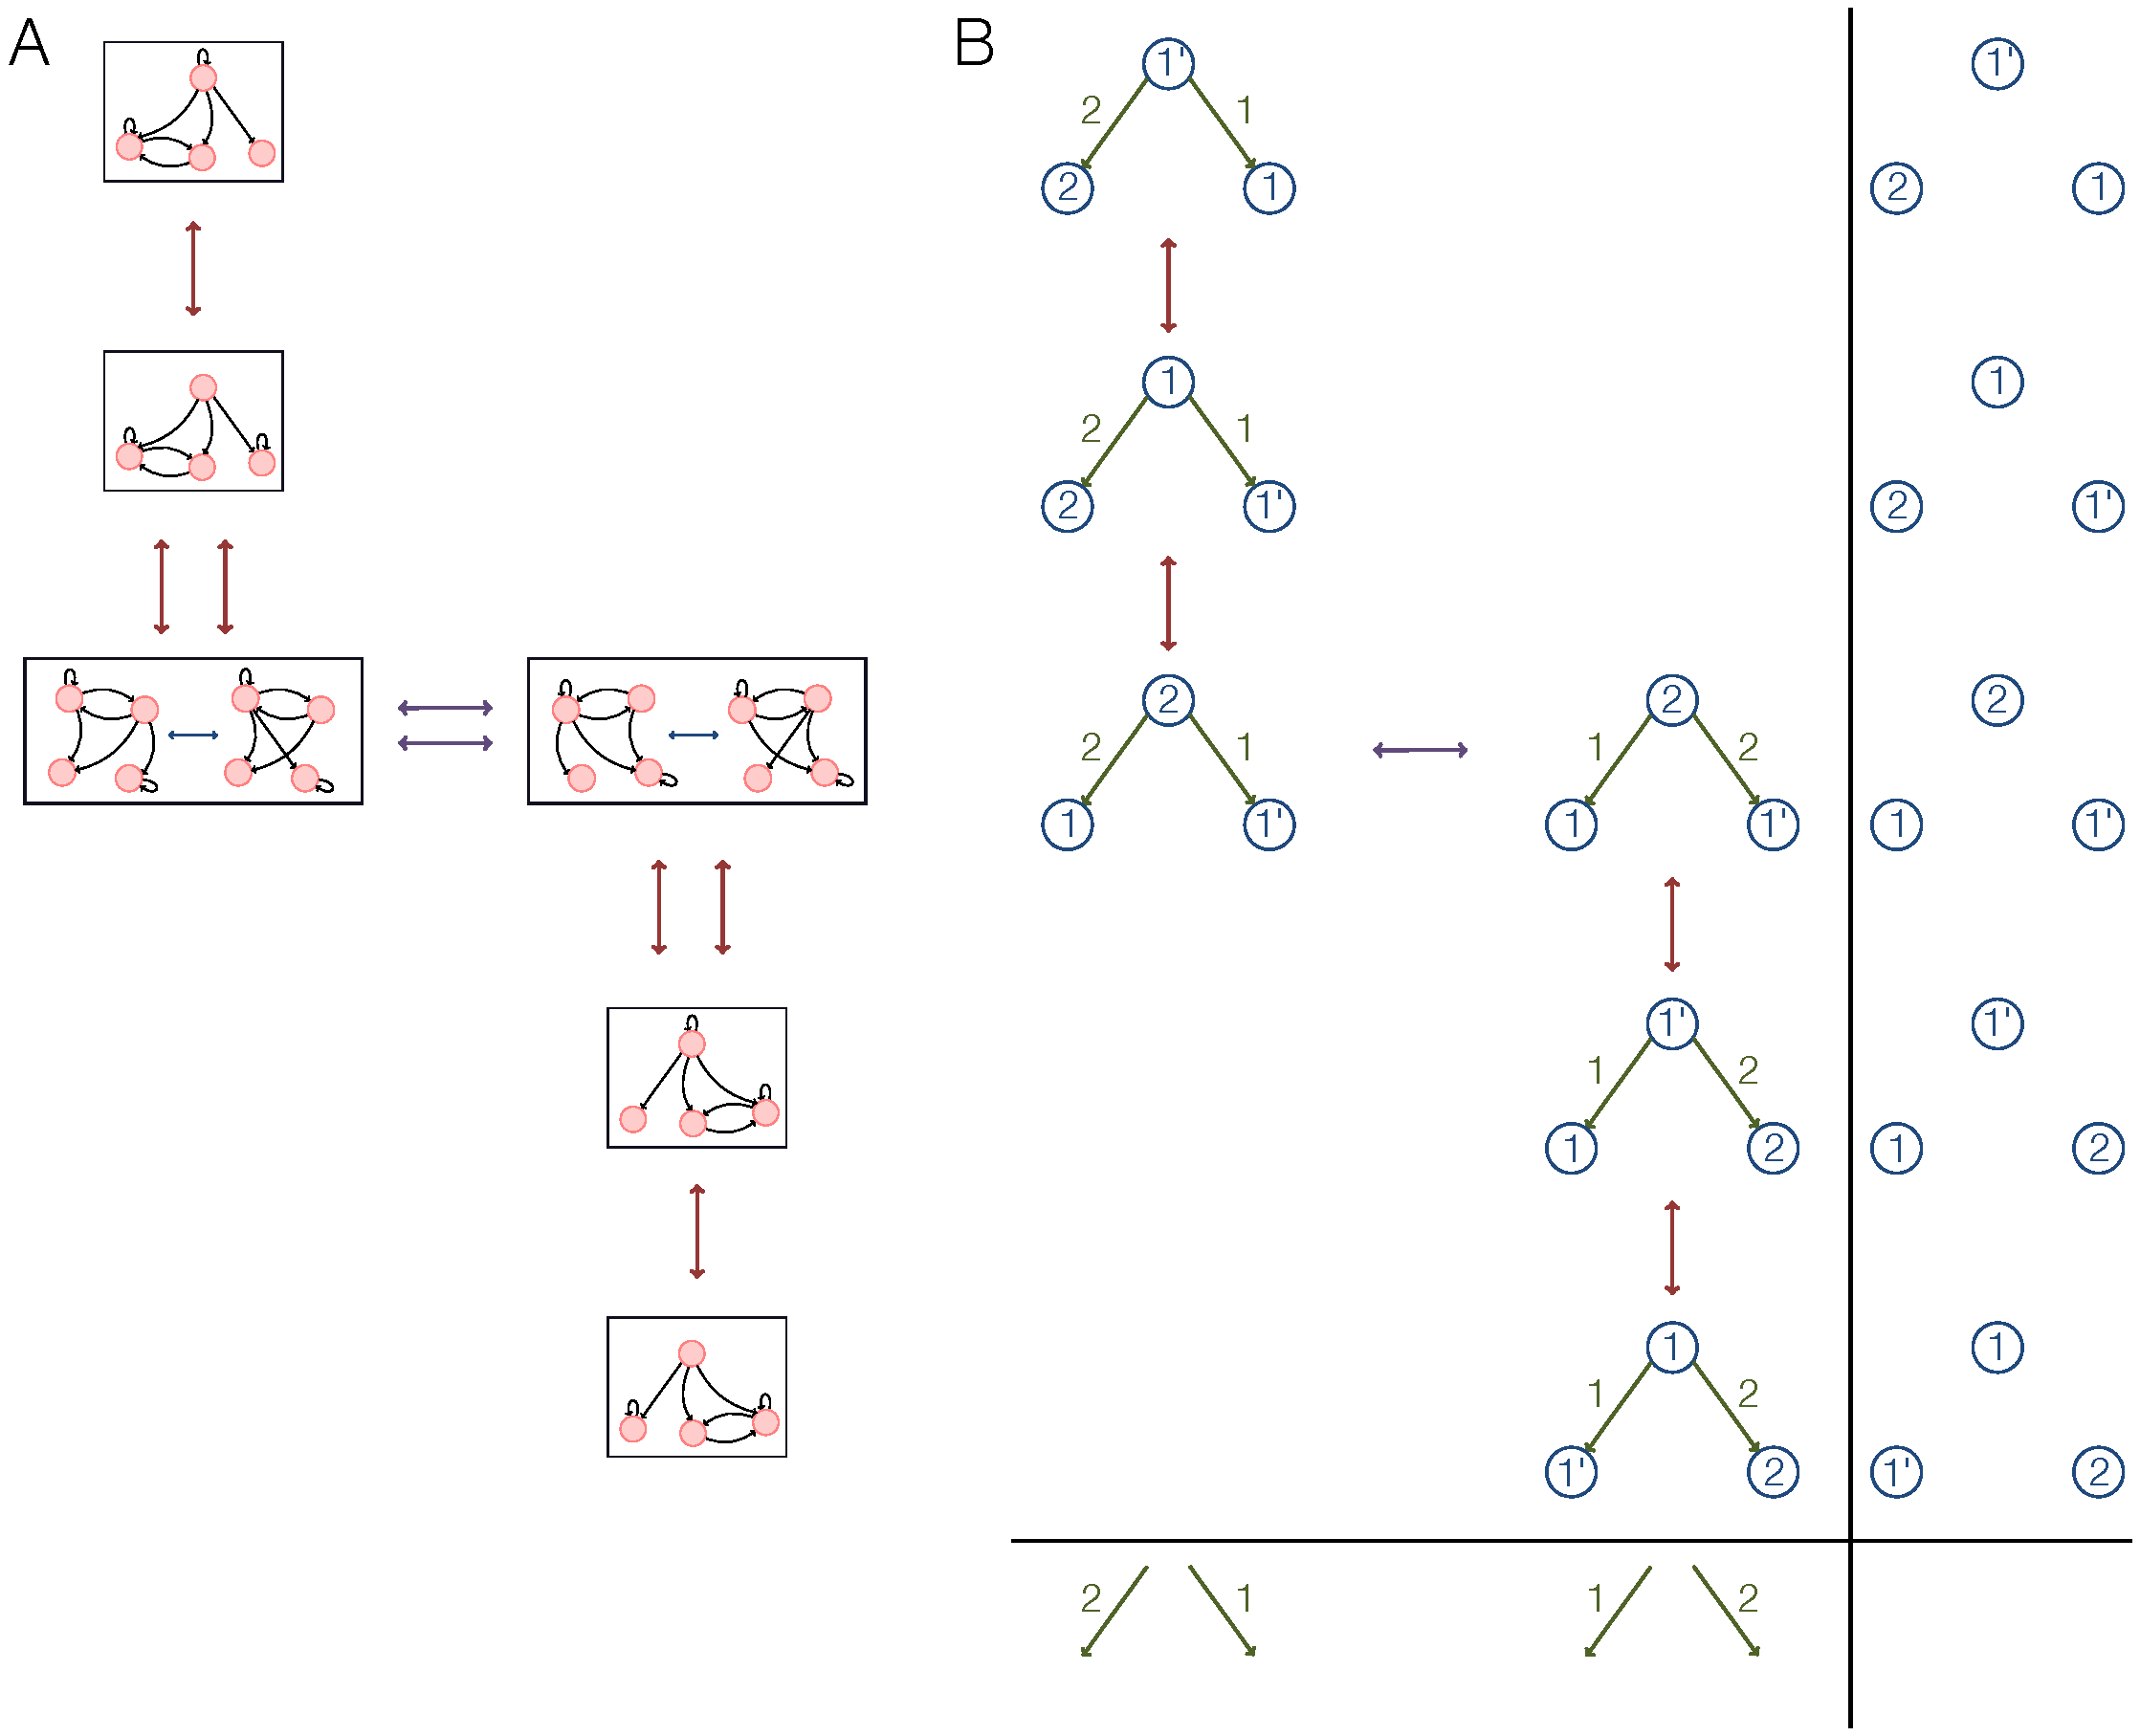
\includegraphics[width=0.9\columnwidth]{fig/robustnesssymmetries.pdf}
\caption{{\bf Example symmetries of robustness.} In this example, the connected component sizes are fixed at $\{2,1,1\}$ with a total of $3$ links between them. Red arrows correspond to transformations like \ref{fig:hiertransformations}A where SCCs are swapped whereas purple arrows correspond to transformations like \ref{fig:hiertransformations}B where links are moved between nodes within a SCC.}
\label{fig:robustnesssymmetries}
\end{figure}

% \begin{figure}[!ht]
% \centering
% \noindent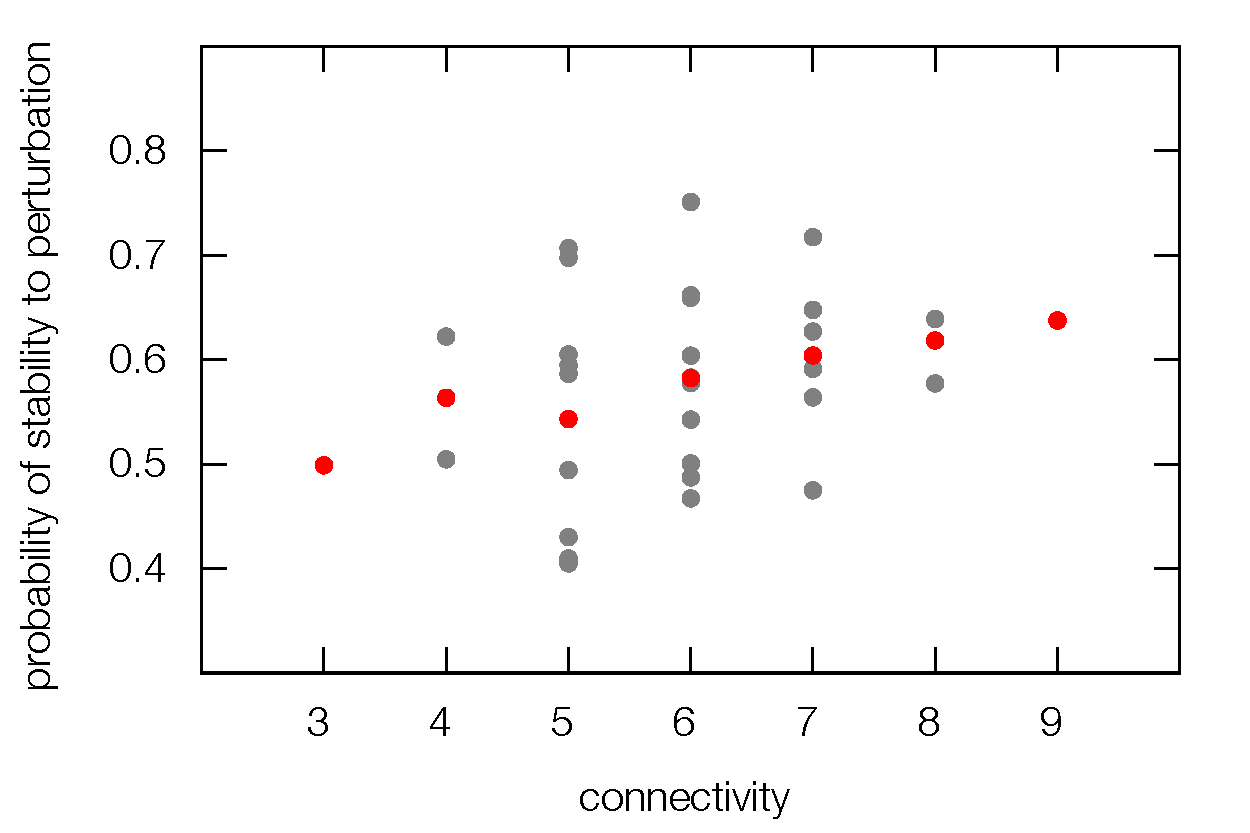
\includegraphics[width=0.8\columnwidth]{fig/stab3x3.pdf}
% \caption{{\bf Plot of stability to perturbations versus connectivity for three component systems.} }
% \label{fig:stab3x3}
% \end{figure}

% \begin{figure}[!ht]
% \centering
% \noindent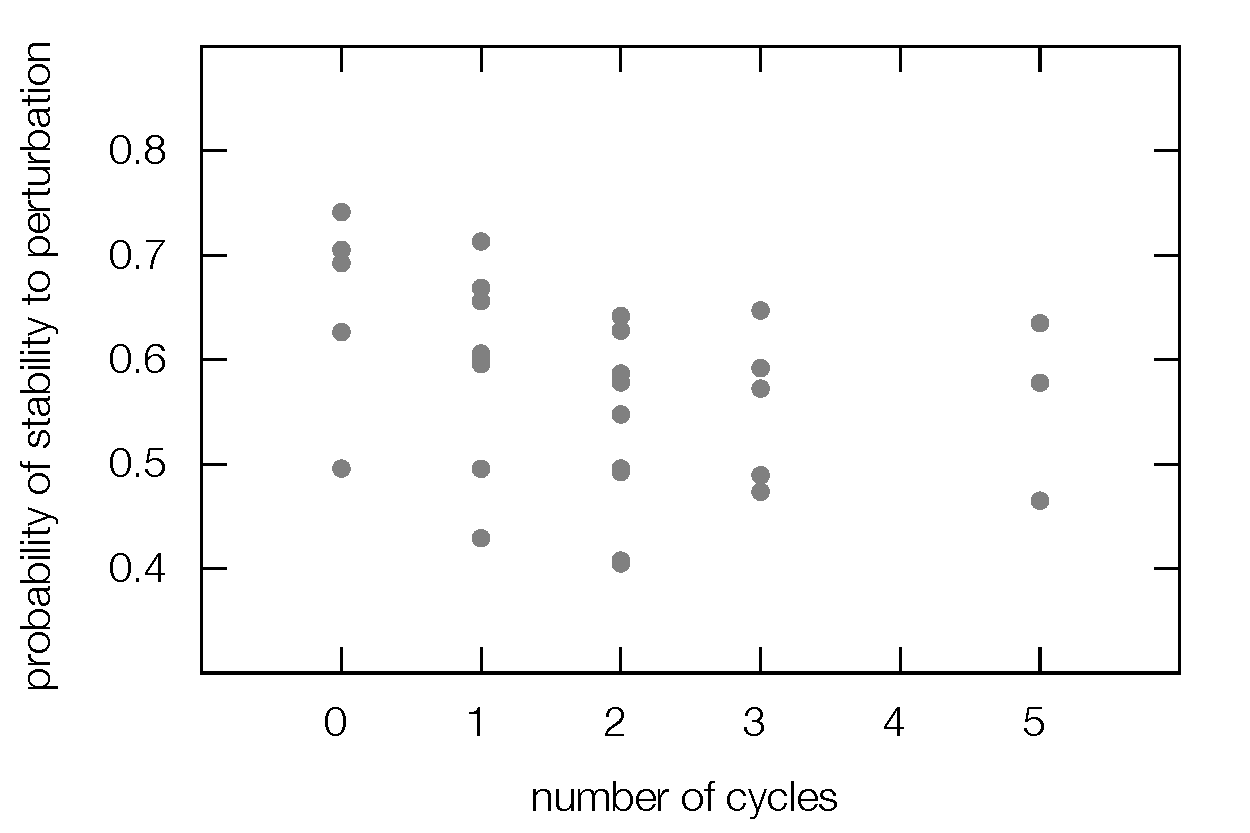
\includegraphics[width=0.8\columnwidth]{fig/cycle3x3.pdf}
% \caption{{\bf Plot of stability to perturbations versus number of cycles for three component systems.} }
% \label{fig:cycle3x3}
% \end{figure}
